\documentclass[aps,pra,amsmath,twocolumn,amssymb,superscriptaddress]{revtex4-1}


\usepackage{amssymb}
\usepackage{amsthm}
\usepackage{amsfonts}
\usepackage{complexity}
\usepackage{graphicx}% Include figure files
\usepackage{dcolumn}% Align table columns on decimal point
\usepackage{bm}% bold math
\usepackage{hyperref}
\usepackage{enumerate}
\usepackage{algorithm}
\usepackage{algpseudocode}
    \renewcommand{\algorithmicrequire}{\textbf{Input:}}
    \renewcommand{\algorithmicensure}{\textbf{Output:}}
    \newcommand{\inlinecomment}[1]{\Comment {\footnotesize #1} \normalsize}
    \newcommand{\linecomment}[1]{\State \(\triangleright\) {\footnotesize #1} \normalsize}
    %\renewcommand{\algorithmiccomment}[1]{\State\(\triangleright\) #1}
    
\usepackage{multirow}

\newtheorem{theorem}{Theorem}
\newtheorem{lemma}{Lemma}
\newtheorem{definition}{Definition}
\newtheorem{corollary}{Corollary}

%    Q-circuit version 2
%    Copyright (C) 2004  Steve Flammia & Bryan Eastin
%    Last modified on: 9/16/2011
%
%    This program is free software; you can redistribute it and/or modify
%    it under the terms of the GNU General Public License as published by
%    the Free Software Foundation; either version 2 of the License, or
%    (at your option) any later version.
%
%    This program is distributed in the hope that it will be useful,
%    but WITHOUT ANY WARRANTY; without even the implied warranty of
%    MERCHANTABILITY or FITNESS FOR A PARTICULAR PURPOSE.  See the
%    GNU General Public License for more details.
%
%    You should have received a copy of the GNU General Public License
%    along with this program; if not, write to the Free Software
%    Foundation, Inc., 59 Temple Place, Suite 330, Boston, MA  02111-1307  USA

% Thanks to the Xy-pic guys, Kristoffer H Rose, Ross Moore, and Daniel Müllner,
% for their help in making Qcircuit work with Xy-pic version 3.8.  
% Thanks also to Dave Clader, Andrew Childs, Rafael Possignolo, Tyson Williams,
% Sergio Boixo, Cris Moore, Jonas Anderson, and Stephan Mertens for helping us test 
% and/or develop the new version.

\usepackage[color]{xy}
\UseCrayolaColors
\xyoption{matrix}
\xyoption{frame}
\xyoption{arrow}
\xyoption{arc}

\usepackage{ifpdf}
\ifpdf
\else
\PackageWarningNoLine{Qcircuit}{Qcircuit is loading in Postscript mode.  The Xy-pic options ps and dvips will be loaded.  If you wish to use other Postscript drivers for Xy-pic, you must modify the code in Qcircuit.tex}
%    The following options load the drivers most commonly required to
%    get proper Postscript output from Xy-pic.  Should these fail to work,
%    try replacing the following two lines with some of the other options
%    given in the Xy-pic reference manual.
\xyoption{ps}
\xyoption{dvips}
\fi

% The following resets Xy-pic matrix alignment to the pre-3.8 default, as
% required by Qcircuit.
\entrymodifiers={!C\entrybox}

%\newcommand{\bra}[1]{{\left\langle{#1}\right\vert}}
%\newcommand{\ket}[1]{{\left\vert{#1}\right\rangle}}
    % Defines Dirac notation. %7/5/07 added extra braces so that the commands will work in subscripts.
\newcommand{\qw}[1][-1]{\ar @{-} [0,#1]}
\newcommand{\eqw}[1][-1]{\ar @{-} @[Red] [0,#1]}
    % Defines a wire that connects horizontally.  By default it connects to the object on the left of the current object.
    % WARNING: Wire commands must appear after the gate in any given entry.
\newcommand{\qwx}[1][-1]{\ar @{-} [#1,0]}
    % Defines a wire that connects vertically.  By default it connects to the object above the current object.
    % WARNING: Wire commands must appear after the gate in any given entry.
\newcommand{\cw}[1][-1]{\ar @{=} [0,#1]}
    % Defines a classical wire that connects horizontally.  By default it connects to the object on the left of the current object.
    % WARNING: Wire commands must appear after the gate in any given entry.
\newcommand{\cwx}[1][-1]{\ar @{=} [#1,0]}
    % Defines a classical wire that connects vertically.  By default it connects to the object above the current object.
    % WARNING: Wire commands must appear after the gate in any given entry.
\newcommand{\gate}[1]{*+<.6em>{#1} \POS ="i","i"+UR;"i"+UL **\dir{-};"i"+DL **\dir{-};"i"+DR **\dir{-};"i"+UR **\dir{-},"i" \qw}
\newcommand{\eboxgate} [1]{*+<.6em>{#1} \POS ="i","i"+UR;"i"+UL **[red]\dir{-};"i"+DL **[red]\dir{-};"i"+DR **[red]\dir{-};"i"+UR **[red]\dir{-},"i" \eqw}
\newcommand{\circgate}[1]{*+<0.6em>[o][F-]{#1} \eqw}
\newcommand{\ecircgate}[1]{*+<0.6em>[o][F-:red]{#1} \eqw}
\newcommand{\filtergt}[1]{\eboxgate{\scriptscriptstyle{#1}}}
\newcommand{\idealdec}{*+<1.2em>{\phantom{*}} \POS ="i","i"+UL;"i"+DL **[red]\dir{-};"i"+R **[red]\dir{-};"i"+UL **[red]\dir{-},"i" \eqw}

    % Boxes the argument, making a gate.
\newcommand{\meter}{*=<1.8em,1.4em>{\xy ="j","j"-<.778em,.322em>;{"j"+<.778em,-.322em> \ellipse ur,_{}},"j"-<0em,.4em>;p+<.5em,.9em> **\dir{-},"j"+<2.2em,2.2em>*{},"j"-<2.2em,2.2em>*{} \endxy} \POS ="i","i"+UR;"i"+UL **\dir{-};"i"+DL **\dir{-};"i"+DR **\dir{-};"i"+UR **\dir{-},"i" \qw}
    % Inserts a measurement meter.
    % In case you're wondering, the constants .778em and .322em specify
    % one quarter of a circle with radius 1.1em.
    % The points added at + and - <2.2em,2.2em> are there to strech the
    % canvas, ensuring that the size is unaffected by erratic spacing issues
    % with the arc.
\newcommand{\measure}[1]{*+[F-:<.9em>]{#1} \qw}
    % Inserts a measurement bubble with user defined text.
\newcommand{\measuretab}[1]{*{\xy*+<.6em>{#1}="e";"e"+UL;"e"+UR **\dir{-};"e"+DR **\dir{-};"e"+DL **\dir{-};"e"+LC-<.5em,0em> **\dir{-};"e"+UL **\dir{-} \endxy} \qw}
    % Inserts a measurement tab with user defined text.
\newcommand{\measureD}[1]{*{\xy*+=<0em,.1em>{#1}="e";"e"+UR+<0em,.25em>;"e"+UL+<-.5em,.25em> **\dir{-};"e"+DL+<-.5em,-.25em> **\dir{-};"e"+DR+<0em,-.25em> **\dir{-};{"e"+UR+<0em,.25em>\ellipse^{}};"e"+C:,+(0,1)*{} \endxy} \qw}
\newcommand{\emeasureD}[1]{*{\xy*+=<0em,.1em>{#1}="e";"e"+UR+<0em,.25em>;"e"+UL+<-.5em,.25em> **[red]\dir{-};"e"+DL+<-.5em,-.25em> **[red]\dir{-};"e"+DR+<0em,-.25em> **[red]\dir{-};{"e"+UR+<0em,.25em>\ellipse{}};"e"+C:,+(0,1)*{} \endxy} \qw}
    % Inserts a D-shaped measurement gate with user defined text.
\newcommand{\multimeasure}[2]{*+<1em,.9em>{\hphantom{#2}} \qw \POS[0,0].[#1,0];p !C *{#2},p \drop\frm<.9em>{-}}
    % Draws a multiple qubit measurement bubble starting at the current position and spanning #1 additional gates below.
    % #2 gives the label for the gate.
    % You must use an argument of the same width as #2 in \ghost for the wires to connect properly on the lower lines.
\newcommand{\multimeasureD}[2]{*+<1em,.9em>{\hphantom{#2}} \POS [0,0]="i",[0,0].[#1,0]="e",!C *{#2},"e"+UR-<.8em,0em>;"e"+UL **\dir{-};"e"+DL **\dir{-};"e"+DR+<-.8em,0em> **\dir{-};{"e"+DR+<0em,.8em>\ellipse^{}};"e"+UR+<0em,-.8em> **\dir{-};{"e"+UR-<.8em,0em>\ellipse^{}},"i" \qw}
    % Draws a multiple qubit D-shaped measurement gate starting at the current position and spanning #1 additional gates below.
    % #2 gives the label for the gate.
    % You must use an argument of the same width as #2 in \ghost for the wires to connect properly on the lower lines.
\newcommand{\control}{*!<0em,.025em>-=-<.2em>{\bullet}}
    % Inserts an unconnected control.
\newcommand{\controlo}{*+<.01em>{\xy -<.095em>*\xycircle<.19em>{} \endxy}}
    % Inserts a unconnected control-on-0.
\newcommand{\ctrl}[1]{\control \qwx[#1] \qw}
    % Inserts a control and connects it to the object #1 wires below.
\newcommand{\ctrlo}[1]{\controlo \qwx[#1] \qw}
    % Inserts a control-on-0 and connects it to the object #1 wires below.
\newcommand{\targ}{*+<.02em,.02em>{\xy ="i","i"-<.39em,0em>;"i"+<.39em,0em> **\dir{-}, "i"-<0em,.39em>;"i"+<0em,.39em> **\dir{-},"i"*\xycircle<.4em>{} \endxy} \qw}
    % Inserts a CNOT target.
\newcommand{\qswap}{*=<0em>{\times} \qw}
    % Inserts half a swap gate.
    % Must be connected to the other swap with \qwx.
\newcommand{\multigate}[2]{*+<1em,.9em>{\hphantom{#2}} \POS [0,0]="i",[0,0].[#1,0]="e",!C *{#2},"e"+UR;"e"+UL **\dir{-};"e"+DL **\dir{-};"e"+DR **\dir{-};"e"+UR **\dir{-},"i" \qw}
    % Draws a multiple qubit gate starting at the current position and spanning #1 additional gates below.
    % #2 gives the label for the gate.
    % You must use an argument of the same width as #2 in \ghost for the wires to connect properly on the lower lines.
\newcommand{\ghost}[1]{*+<1em,.9em>{\hphantom{#1}} \qw}
    % Leaves space for \multigate on wires other than the one on which \multigate appears.  Without this command wires will cross your gate.
    % #1 should match the second argument in the corresponding \multigate.
\newcommand{\push}[1]{*{#1}}
    % Inserts #1, overriding the default that causes entries to have zero size.  This command takes the place of a gate.
    % Like a gate, it must precede any wire commands.
    % \push is useful for forcing columns apart.
    % NOTE: It might be useful to know that a gate is about 1.3 times the height of its contents.  I.e. \gate{M} is 1.3em tall.
    % WARNING: \push must appear before any wire commands and may not appear in an entry with a gate or label.
\newcommand{\gategroup}[6]{\POS"#1,#2"."#3,#2"."#1,#4"."#3,#4"!C*+<#5>\frm{#6}}
    % Constructs a box or bracket enclosing the square block spanning rows #1-#3 and columns=#2-#4.
    % The block is given a margin #5/2, so #5 should be a valid length.
    % #6 can take the following arguments -- or . or _\} or ^\} or \{ or \} or _) or ^) or ( or ) where the first two options yield dashed and
    % dotted boxes respectively, and the last eight options yield bottom, top, left, and right braces of the curly or normal variety.  See the Xy-pic reference manual for more options.
    % \gategroup can appear at the end of any gate entry, but it's good form to pick either the last entry or one of the corner gates.
    % BUG: \gategroup uses the four corner gates to determine the size of the bounding box.  Other gates may stick out of that box.  See \prop.

\newcommand{\rstick}[1]{*!L!<-.5em,0em>=<0em>{#1}}
    % Centers the left side of #1 in the cell.  Intended for lining up wire labels.  Note that non-gates have default size zero.
\newcommand{\lstick}[1]{*!R!<.5em,0em>=<0em>{#1}}
    % Centers the right side of #1 in the cell.  Intended for lining up wire labels.  Note that non-gates have default size zero.
\newcommand{\ustick}[1]{*!D!<0em,-.5em>=<0em>{#1}}
    % Centers the bottom of #1 in the cell.  Intended for lining up wire labels.  Note that non-gates have default size zero.
\newcommand{\dstick}[1]{*!U!<0em,.5em>=<0em>{#1}}
    % Centers the top of #1 in the cell.  Intended for lining up wire labels.  Note that non-gates have default size zero.
\newcommand{\Qcircuit}{\xymatrix @*=<0em>}
    % Defines \Qcircuit as an \xymatrix with entries of default size 0em.
\newcommand{\link}[2]{\ar @{-} [#1,#2]}
    % Draws a wire or connecting line to the element #1 rows down and #2 columns forward.
\newcommand{\pureghost}[1]{*+<1em,.9em>{\hphantom{#1}}}
    % Same as \ghost except it omits the wire leading to the left. 
%%%%%%%%%%%%%%%%%%%%%%%%%%%%%%%%%%%%%%%%%%%%%%%%%%%%%%%%%%%%%%%%%%%%%%%%%%%%%%%%%%%%%%%%%%
\newcommand{\multiprepareC}[2]{*+<1em,.9em>{\hphantom{#2}}\save[0,0].[#1,0];p\save !C
  *{#2},p+RU+<0em,0em>;+LU+<+.8em,0em> **\dir{-}\restore\save +RD;+RU **\dir{-}\restore\save
  +RD;+LD+<.8em,0em> **\dir{-} \restore\save +LD+<0em,.8em>;+LU-<0em,.8em> **\dir{-} \restore \POS
  !UL*!UL{\cir<.9em>{u_r}};!DL*!DL{\cir<.9em>{l_u}}\restore}
   % Draws a multiple qubit reverse-D-shaped preparation gate starting at the current position and spanning #1 additional gates below.
   % #2 gives the label for the gate.
   % You must use an argument of the same width as #2 in \pureghost for the wires to connect properly on
% the lower lines.
\newcommand{\prepareC}[1]{*{\xy*+=+<.5em>{\vphantom{#1\rule{0em}{.1em}}}*\cir{l^r};p\save*!L{#1} \restore\save+UC;+UC+<.5em,0em>*!L{\hphantom{#1}}+R **\dir{-} \restore\save+DC;+DC+<.5em,0em>*!L{\hphantom{#1}}+R **\dir{-} \restore\POS+UC+<.5em,0em>*!L{\hphantom{#1}}+R;+DC+<.5em,0em>*!L{\hphantom{#1}}+R **\dir{-} \endxy}}
   % Inserts a reverse-D-shaped preparation gate with user defined text.
\newcommand{\poloFantasmaCn}[1]{{{}^{#1}_{\phantom{#1}}}}



\def\ket#1{\left|#1\right\rangle}
\def\bra#1{\langle#1|}
\newcommand{\ketbra}[2]{|#1\rangle\!\langle#2|}
\newcommand{\braket}[2]{\langle#1|#2\rangle}
% \newcommand{\note}[1]{({\bf note: #1})}
\newcommand{\prob}[1]{{\rm Pr}\left(#1 \right)}
% \newcommand{\Tr}[1]{{\rm Tr}\!\left[#1 \right]}
\newcommand{\expect}[2]{{\mathbb{E}_{#2}}\!\left\{#1 \right\}}
\newcommand{\var}[2]{{\mathbb{V}_{#2}}\!\left\{#1 \right\}}
\newcommand{\CRej}{\text{RejS }}

\newcommand{\sinc}{\operatorname{sinc}}

% fix: supported only for revtex
%\newcommand{\openone}{\mathbb{I}}
% fix: unsupported with iopart
%\newcommand{\eqref}[1]{(\ref{#1})}

\newcommand{\sde}{\mathrm{sde}}
\newcommand{\Z}{\mathbb{Z}}
\newcommand{\RR}{\mathbb{R}}
\newcommand{\w}{\omega}
\newcommand{\Kap}{\kappa}

\newcommand{\Tchar}{$T$}
\newcommand{\T}{\Tchar~}
\newcommand{\TT}{\mathrm{T}}
\newcommand{\ClT}{\{{\rm Clifford}, \Tchar\}~}
\newcommand{\Tcount}{\Tchar--count~}
\newcommand{\Tcountper}{\Tchar--count}
\newcommand{\Tcounts}{\Tchar--counts~}
\newcommand{\Tdepth}{\Tchar--depth~}
\newcommand{\Zr}{\Z[i,1/\sqrt{2}]}
\newcommand{\ve}{\varepsilon}

\newcommand{\eq}[1]{\hyperref[eq:#1]{(\ref*{eq:#1})}}
\renewcommand{\sec}[1]{\hyperref[sec:#1]{Section~\ref*{sec:#1}}}
\newcommand{\app}[1]{\hyperref[app:#1]{Appendix~\ref*{app:#1}}}
\newcommand{\fig}[1]{\hyperref[fig:#1]{Figure~\ref*{fig:#1}}}
\newcommand{\thm}[1]{\hyperref[thm:#1]{Theorem~\ref*{thm:#1}}}
\newcommand{\lem}[1]{\hyperref[lem:#1]{Lemma~\ref*{lem:#1}}}
\newcommand{\tab}[1]{\hyperref[tab:#1]{Table~\ref*{tab:#1}}}
\newcommand{\cor}[1]{\hyperref[cor:#1]{Corollary~\ref*{cor:#1}}}
\newcommand{\alg}[1]{\hyperref[alg:#1]{Algorithm~\ref*{alg:#1}}}
\newcommand{\defn}[1]{\hyperref[def:#1]{Definition~\ref*{def:#1}}}


\newcommand{\targfix}{\qw {\xy {<0em,0em> \ar @{ - } +<.39em,0em>
\ar @{ - } -<.39em,0em> \ar @{ - } +
<0em,.39em> \ar @{ - }
-<0em,.39em>},<0em,0em>*{\rule{.01em}{.01em}}*+<.8em>\frm{o}
\endxy}}

\newenvironment{proofof}[1]{\begin{trivlist}\item[]{\flushleft\it
Proof of~#1.}}
{\qed\end{trivlist}}


\newcommand{\cu}[1]{{\textcolor{red}{#1}}}
\newcommand{\tout}[1]{{}}
% \newcommand{\beq}{\begin{equation}}
% \newcommand{\eeq}{\end{equation}}
% \newcommand{\beqa}{\begin{eqnarray}}
\newcommand{\good}{{\rm good}}
\newcommand{\bad}{{\rm bad}}
% \newcommand{\eeqa}{\end{eqnarray}}

\newcommand{\id}{\openone}
%\newcommand{\id}{\mathbb{I}}

\newcommand{\etal}{\emph{et al}}
\newcommand{\ii}{\mathrm{i}}
\newcommand{\ee}{\mathrm{e}}

%%%%%%%%%%%%%%%%%%%%%%% a bit nicer hypelinks %%%%%%%%%%%%%%%%%%%%%%%%%%%%%

\usepackage[usenames,dvipsnames]{xcolor}
\hypersetup{
    colorlinks=true,       % false: boxed links; true: colored links
    linkcolor=Maroon,          % color of internal links (change box color with linkbordercolor)
    citecolor=OliveGreen,        % color of links to bibliography
    filecolor=magenta,      % color of file links
    urlcolor=Blue           % color of external links
}

%%%%%%%%%%%%%%%%%%%%%%% a bit nicer hypelinks %%%%%%%%%%%%%%%%%%%%%%%%%%%%%

\begin{document}

%=============================================================================
% FRONT MATTER
%=============================================================================

\title{Efficient Bayesian Phase Estimation}
\author{Nathan Wiebe}
\affiliation{Quantum Architectures and Computation Group, Microsoft Research, Redmond, WA (USA)}

\author{Chris Granade}
\affiliation{Centre for Engineered Quantum Systems, Sydney, NSW (Australia)}
\affiliation{School of Physics, University of Sydney, Sydney, NSW (Australia)}

\begin{abstract}
    We provide a new method for performing phase estimation using adaptive
    Bayesian inference and rejection sampling.  Our method not only yields
    comparable performance to iterative phase estimation in absentia of
    decoherence, but also continues to work without modification when
    decoherence or other imperfections are present.  Furthermore, our method
    is trivial to apply in any experimental system that is already capable of
    running iterative phase estimation experiments. This work not only shows that
 decoherence is not a
    fundamental limitation to our ability to learn eigenvalues and that ideas
    from computer vision and statistical inference can be leveraged to reveal
    new classes of efficient phase estimation algorithms that are more broadly
    applicable than existing methods.
\end{abstract}

\maketitle

%=============================================================================
\section{Introduction}
\label{sec:intro}
%=============================================================================

Phase estimation is a technique of fundamental importance to quantum information.  Phase estimation provides a method to efficiently compute the eigenphase corresponding to an input eigenstate of a unitary $U$ within a user specified precision.  The protocol typically forms the core of quantum simulation algorithms, linear systems algorithms or and the amplitude estimation algorithm.  As a result, methods that even modestly improve the time and space complexities of phase estimation or increase the algorithm's robustness to experimental errors are of great importance because they can allow sophisticated examples of such algorithms to be executed without the need for a fault tolerant quantum computer.

Iterative phase estimation seeks to learn the eigenvalue of a given
eigenvector of $U$ using a classical inference algorithm run in conjunction
with a simple quantum circuit to infer the bits of a binary expansion of the
phase.  Iterative phase estimation is typically used in preference to
traditional phase estimation because its simplicity and minimal qubit
requirements

The quantum circuit used in iterative phase estimation is~\cite{SHF14}
\begin{equation}
    \nonumber
    \Qcircuit @C=1em @R=1em {
        \lstick{\ket{0}}    & \gate{H}  & \gate{Z(-M \theta)}   & \ctrl{1}   & \gate{H} & \meter & \cw \\
        \lstick{\ket{\phi}} & {/} \qw   & \qw                   & \gate{U^M} & \qw      & \qw    & \qw
    }
\end{equation}
where $U\ket{\phi} = \ee^{\ii\phi}\ket{\phi}$ for an unknown eigenphase $\phi \in \mathbb{R}$,
and where $Z(M \theta) = \ee^{\ii M \theta Z}$ is a rotation used to approximately invert $U^M$.
The most commonly used method for performing iterative phase estimation uses this circuit to learn the bits
of $\phi$ in order from least significant to most significant.  The process is near optimal (up to $\log^*$ factors) and
affords a classically efficient and deterministic process for inferring these bits.

A drawback to iterative phase estimation is that it is not necessarily robust to experimental errors.  This is because the inference process used to find the bits of the unknown phase  is specialized for the probability distribution induced by an ideal phase estimation experiment, which may not accurately model that yielded by an imperfect implementation.  This issue becomes
particularly significant as more bits of precision are required since typical phase estimation algorithms require that $M$ grow exponentially.
This means that initially weak decoherence eventually becomes a major impediment to our ability to learn an unknown eigenphase
through phase estimation.  

Bayesian methods proposed by Svore \etal~\cite{SHF14} are not as susceptable
to these problems, as they do not require that the user chooses a particular
sequence of $M$. Despite this, existing proposals for performing Bayesian
phase estimation require an exponential amount of processing time to process
the data from the experiments and also may suffer from the use of randomly
chosen experiments in cases where a continuum of eigenphases are possible.

Our work addresses these problems by not only providing a method for
performing an efficient form of Bayesian phase estimation but also giving an
expedient heuristic for adaptively choosing approximately optimal experiments.
We illustrate this by showing that our algorithm not only exhibits the same
Heisenberg limited scaling of phase estimation in decoherence--free cases but
continues to learn even when decoherence would ordinarily prevent traditional phase estimation
methods from working.

%=============================================================================
\section{Bayesian Phase Estimation}
\label{sec:bayesian-phase-est}
%=============================================================================

In order to understand how our algorithm works it is important to discuss how
exact Bayesian phase estimation operates. The idea behind Bayesian phase
estimation is to use Bayes' rule to estimate the most probable eigenphase given
a set of experimental data. It keeps track of the probability that a
particular eigenphase, $\phi$, is the correct phase using a \emph{prior
distribution}. The initial prior distribution is subjective, but it is
customarily taken to be flat unless the user has strong reason to suspect that
some eigenphases are more probable than others. Importantly, Bayesian inference
can recover from bad prior distributions at the cost of additional
experiments, provided the true eigenphase is supported by the initial prior.

The inference process of Svore \etal~\cite{SHF14} involves performing a random
set of experiments and then updating the prior distribution using Bayes' rule.
For example, if an experiment is performed with using $M$ repetitions of $U$,
$Z(M \theta)$ and a measurement outcome $E\in \{0,1\}$ is observed then Bayes'
rule states that the \emph{posterior probability} distribution for $\phi$
after observing the datum is
\begin{equation}
P(\phi|E;\theta,M) = \frac{P(E|\phi;\theta,M)P(\phi)}{\int P(E|\phi;\theta,M)P(\phi)\mathrm{d}{\phi}}.\label{eq:update}
\end{equation}
The final ingredient that is needed to perform an update is the likelihood function, $P(0|\phi;\theta,M)$, is easy to compute for phase estimation:
\begin{gather}
    \label{eq:likenodecohere}
    \begin{aligned}
        P(0|\phi;\theta,M) & = \frac{1+\cos(M[\phi +\theta])}{2},\\
        P(1|\phi;\theta,M) & = \frac{1-\cos(M[\phi +\theta])}{2}.
    \end{aligned}
\end{gather}
After using~\eq{update} to update the posterior distribution we then set the prior distribution to equal the posterior distribution.  This process is then repeated for each of the random experiments in the data set.

Unlike conventional methods, Bayesian inference returns a posterior distribution over the
phase An estimate of and uncertianty in the phase is extracted from the
posterior distribution, usually as the mean and variance of the posterior,
respectively. More sophisticated estimates of uncertainty, such as credible
regions, can also be easily extracted from the posterior
distribution~\cite{granade_robust_2012}.  This estimate of the uncertainty is
vital for these algorithms because it not only gives the confidence in the
result but also provides a stopping criteria.  Since iterative phase
estimation requires that you learn the bits in reverse order, this feature is
significant because it allows the user to prematurely end the inference once
an accuracy target has been met.

\begin{figure}[t!]
    \begin{centering}
        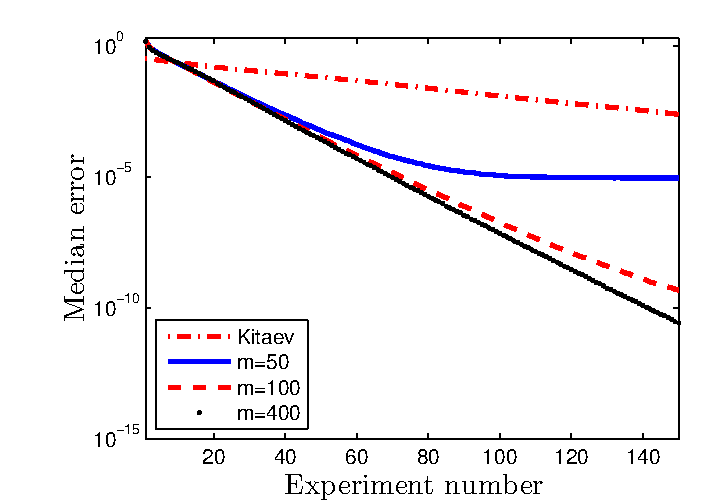
\includegraphics[width=0.8\linewidth]{PEerror.pdf}
    \end{centering}
    \caption{\label{fig:PEerror}
     Median errors in phase estimation for 10~000 random initial choices of the true eigenphase.
% and initial prior is taken to be uniform.
    }
\end{figure}


\section{Approximate Bayesian Phase Estimation}
The major drawback of Bayesian PE is that there are an infinite number of hypotheses in the prior.  Our method addresses this by updating a model for the posterior distribution, rather than the underlying distribution itself.  We do this by assuming a Gaussian model for our initial prior, perform a Bayesian update on samples drawn from the distribution and then refit the updated samples to a Gaussian.  This strategy is commonly used in a number of particle filter approximations to the posterior such as the extended Kalman filter, assumed density filtering or sequential Monte Carlo methods.

These methods, although efficient, can require tracking several thousand
discrete hypotheses for $\phi$ and are hard to implement.  For this reason, we
propose using a much simpler approach that uses rejection sampling to perform
Bayesian inference.  The procedure is as follows.

\begin{figure*}
    \begin{centering}
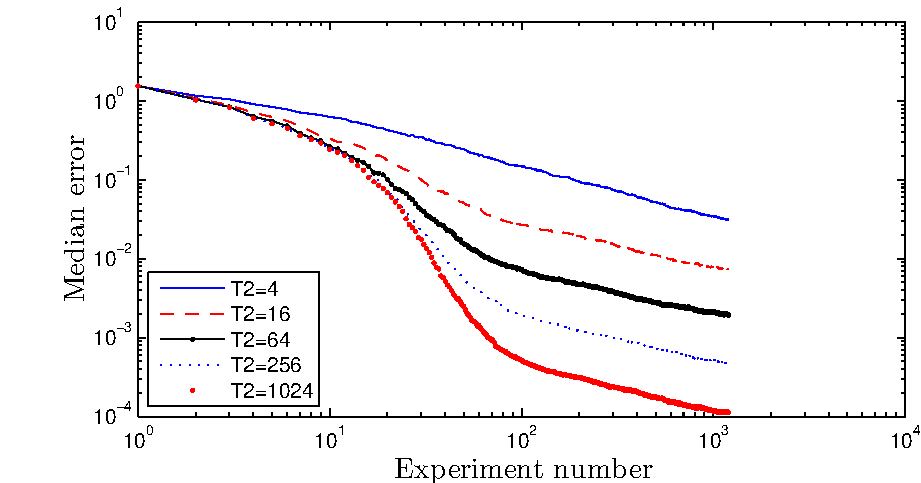
\includegraphics[width=0.45\linewidth]{T2plot_full.pdf}
        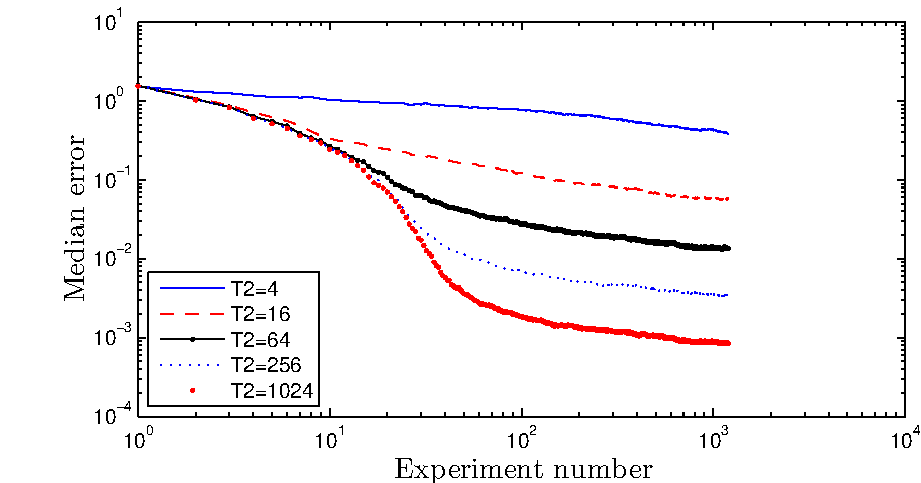
\includegraphics[width=0.45\linewidth]{T2plot.pdf}
    \end{centering}
    \caption{\label{fig:T2plot}
Median errors for phase estimation in decohering systems for experiments constrained to use $M\le T_2$ (left) and $M\le T_2/10$ (right).  We take $m=12~000$ and use $1~000$ random samples to generate the data above.  The initial state is taken to be a fixed but unknown eigenstate in all cases.
    }
\end{figure*}

\begin{enumerate}
\item Perform experiment for given $\theta$, $M$ and observe outcome $E\in \{0,1\}$.
\item Draw $m$ samples from $\mathcal{N}(\mu,\sigma^2)$.
\item For each sample, $\phi_j$, assign $\phi_j$ to $\Phi_{\rm accept}$ with probability $P(E|\phi_j;\theta,M)/\kappa_E$, where $\kappa_E\in (0,1]$ is a constant s.t. $P(E|\phi_j;\theta,M)/\kappa_E\le 1$ for all $\phi_j,E$.
\item Return $\mu = \mathbb{E}(\Phi_{\rm accept})$ and $\sigma =\sqrt{\mathbb{V}(\Phi_{\rm accept})}$.
\end{enumerate}

The samples drawn from this distribution are sampled according to the posterior distribution
$P(\phi|E;M,\theta)$.  To see this, note that the probability density of a sample being accepted at $\phi=\phi_j$ is the product of the probability of acceptance and the probability density of drawing the sample from $\mathcal{N}(\mu,\sigma^2)=P(\phi)$.  Eqn~\eq{update} then implies that
\begin{equation}
    P(E | \phi; \theta, M) \mathcal{N}(\mu,\sigma^2) \propto P(\phi | E; \theta, M).
\end{equation}
Thus the distribution of the accepted samples is equivalent to the posterior distribution.  


The main issue that remains is how to optimally choose the parameters $\theta$ and $M$ to minimize the number of experiments needed to infer the unknown eigenphase $\phi$.
This issue can be solved by local optimization of the risk function, but the resulting calculation can be too expensive to carry out in online experiments that provide experimental results at a rate of tens of Megahertz or faster.  Fortunately, there is an expedient guess heuristic, known as the particle guess heuristic (PGH) that can be used to choose a near optimal experiment for this class of likelihood functions~\cite{wiebe_hamiltonian_2014}.  Specifically we take
\begin{align}
M &= \left\lceil\frac{1.25}{\sigma}\right\rceil,~
\theta \sim P(\phi).\label{eq:PGH}
\end{align}
Here the constant factor of $1.25$ comes from optimizating the median performance of the guess heuristic to the problem of phase estimation.  
$M$ need not be an integer in cases where fractional applications of $U$ are practical, such as quantum simulation.

%A small technical complication emerges because the likelihood function possesses branch cuts.  For example, the sample variance from the Gaussian $\mathcal{N}(0,1)$ will with high probability be much greater than that from $\mathcal{N}(\pi,1)$ if the results are folded into the interval $[0,2\pi]$.  This can be addressed by shifting the interval to remove this illusionary source of variance.

%$M$ does not need to be an integer in general.  In quantum simulation experiments where $U=e^{-iHt}$, fractional powers of the unitary can be executed %without incurring additional quantum cost.  It can be useful to ignore the ceiling function in~\eq{PGH}.

We illustrate the performance of this algorithm in~\fig{PEerror} wherein we plot the median error in phase estimation using our approach (for non--integer $M$ and using a non--incremental formula for the standard deviation).  The most obvious feature is that we observe Heisenberg limitted scaling for $m>100$, meaning that the error shrinks exponentially with the number of experiments (which is proportional to the evolution time under the PGH).  Roughly $150$ experiments are needed for the method to provide $32$ bits of accuracy in the median case.
We discuss the scaling in the mean in the appendix.

The number of experiments needed to reach error $\epsilon$ scales as $O(\log(1/\epsilon))$ rather than $O(\log(1/\epsilon)\log\log(1/\epsilon))$ as per iterative phase estimation.  This illustrates that our adaptive approach can yield substantial performance advantages over existing methods for phase estimation.  Although the number of experiments needed is small, the experimental time required to achieve this is not necessarily small.  Given that the error shrinks as $\epsilon\in \Theta(e^{-\lambda N})$ where $N$ is the experiment number then $T_{\exp}\in O(\sum_{N=1}^{N_{\rm max}}e^{\lambda N})\in O(e^{\lambda N_{\rm max}})\in O(1/\epsilon)$.  Thus the total experimental time required saturates the Heisenberg limit, up to a multiplicative constant.

%We propose the following simple algorithm for phase estimation:





\begin{figure*}
    \begin{centering}
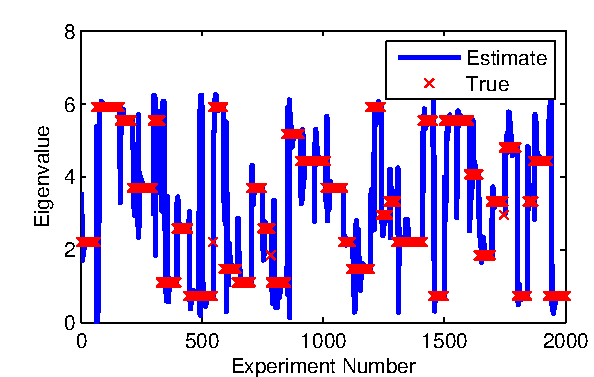
\includegraphics[width=0.4\linewidth]{Errtrack1.pdf}
\hspace{5mm}
        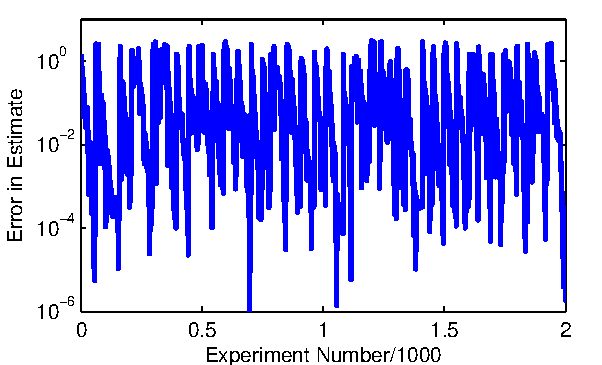
\includegraphics[width=0.4\linewidth]{Errtrack2.pdf}
    \end{centering}
    \caption{\label{fig:Errplot}
Tracking the current estimate of an eigenphase  during phase estimation for a system with $16$ eigenvalues and $T_2=10^4$.
    }
\end{figure*}

\subsection{Phase estimation with depolarizing noise}
A criticism that has been levied lately at the phase estimation algorithm is that it can be impractical to execute on non--fault tolerant quantum hardware.  This is because phase estimation attains its quadratic advantage over statistical sampling by using exponentially long evolutions.  Decoherence causes the resultant phases to become randomized as time progresses, ultimately resulting in
$\lim_{M\rightarrow \infty} P(0|\phi;\theta,M) = \frac{1}{2}$.
In this limit, the measurements convey no information and inference becomes impossible.  It is possible, however, to use our inference method to continue to use phase estimation long after the onset of decoherence.  This observation is exactly analogous to the frequency estimation method presented in~\cite{granade_robust_2012}, which uses particle filter methods to infer an unknown frequency parameter for a small quantum system in the presence of uncharacterized decoherence.

We model the effect of decoherence on the system by assuming the existence of a \emph{decoherence time} $T_2$ such that
\begin{gather}
    \label{eq:likedecohere}
    \begin{aligned}
        P(0|\phi) & = \ee^{-M/T_2}\left(\frac{1+\cos(M[\phi -\theta])}{2}\right)+\frac{1-\ee^{-M/T_2}}{2},\\
        P(1|\phi) & = \ee^{-M/T_2}\left(\frac{1-\cos(M[\phi -\theta])}{2}\right)+\frac{1-\ee^{-M/T_2}}{2}.
    \end{aligned}
\end{gather}
In the limit as $T_2\rightarrow \infty$ the likelihood function~\eq{likedecohere} approaches~\eq{likenodecohere}.  Similarly as $T_2\rightarrow 0$ the likelihood function approaches the uniform distribution.  This model is appropriate when the time required to implement the controlled operation $\Lambda(U)$ is long relative the that required to perform $H$ and an arbitrary $Z$--rotation, as is appropriate in quantum simulation.  For simplicity, in the following we will assume that $T_2$ is well characterized. 


The information provided by each experiment shrinks exponentially with $M$ and hence it is important to choose $M$ differently than one would choose it using the ordinary PGH.  The best approach, suggested in~\cite{granade_robust_2012}, is to adaptively design experiments that minimize the Bayes risk given a prior distribution over $T_2$.  In practice, this can be very expensive given that data is often collected at a rates of $1~{\rm MHz}$ or greater in existing experiments.  This means waiting for a locally optimal experiment means ignoring a prohibitive amount of data even if the optimization requires only a millisecond.  For this reason we propose a variation to \eq{PGH}:
\begin{equation}
M=\min\left\{\left\lceil\frac{1.25}{\sigma}\right\rceil, T_2 \right\}.
\end{equation}
This heuristic is chosen to be qualitatively similar to optimized solutions for
frequency estimation, which are chosen to saturate the Cram\'er-Rao bound \cite{ferrie_how_2013}.
This can be seen through the following argument.  The Cram\'er-Rao bound scales as $O(M^{-2})$ for phase estimation~\cite{WGC15} in the absence of decoherence.  Eqn.~\eq{likedecohere} suggests that depolarizing noise causes the variance to increase as $O(\exp(2M/T_2))$.  Calculus reveals that $M=T_2$ yields an optimal trade off between the two tendencies, as also observed in~\fig{T2plot}.

%An exponential distribution is chosen rather than a
%Gaussian because the exponentially shrinking probability more closely matches
%the exponentially decaying signal expected from experiments with duration much
%greater than $T_2$.  Randomization in this form is useful because it helps
%fight the algorithm becoming stuck in cases where the posterior variance
%underestimates the error.   

The same methodology also applies to the case where
$T_2$ is unknown and can easily be seen from the discussion
in Granade \etal~\cite{granade_robust_2012}.  The only modification needed is that the $T_2$
used in the determination of $M$ should also be drawn from the prior
$P(\phi,T_2)$.




There are several issues that need to be considered in order to make this approach practical.  The first issue that arises in these cases is that since we cannot increase the evolution time without limit, the likelihood function begins to flatten.  This creates an issue because the statistical fluctuations in the calculation in $\mu$ and $\sigma$ can easily be equivalent to the effect of the Bayesian update unless $m$ is large.  In particular, the update process becomes asymptotically unstable if $m \in \Omega(1/\delta^2)$ where $\delta$ is the maximum size of fluctuations of $P(E|\phi)$.  This can be understood by noting that the error in the mean of the accepted samples is $\Theta(1/\sqrt{m})$.  The reduction in the uncertainty in the posterior distribution after an experiment is proportional to $\delta$ if the prior distribution is Gaussian.  Thus if $m\in \Omega(1/\delta^2)$ then the sample noise in $\mu$ is greater than the reduction in $\sigma$, leading to instability.  Either $m$ must be increased or several experiments must be batched together to increase $\delta$  to address these issues. 

The second issue is that, without modification, the probability that a given hypothesis survives $p$ rounds of rejection sampling step shrinks exponentially with $p$.  This can be combatted by taking
\begin{equation}
\kappa_E = \frac{1+e^{-M/T_2}}{2},
\end{equation}
which makes the probability of accepting a sample $1$ if $\theta = \phi_{\rm true}$ even when $T_2\not\gg M$. 

\fig{T2plot} shows that our algorithm smoothly interpolates between the Heisenberg limited scaling expected at short times and continues to learn (albeit only at a polynomial rate) when decoherence becomes significant.  This illustrates that the presence of decoherence does not impose a fundamental limitation on the accuracy that we can achieve in phase estimation and that our approach.  Additionally, we see that forcing the experiments to stay in a more coherent regime can actually hurt the algorithm's ability to infer the phase as expected.

\section{Tracking Eigenphases}
The data in~\fig{T2plot} is appropriate when the initial quantum state is an eigenstate and is discarded after each experiment.  Performing phase estimation in this way minimizes the number of experiments, but can be prohibitively expensive if preparation of the initial eigenstate is prohibitively costly.  Instead, it makes sense to follow the standard prescription for phase estimation by keeping the quantum state until it is clear that the initial eigenstate has been depolarized.  This approach can also be used when $T_2=0$ to cope with cases where the input state is a superposition of eigenvectors or when the learning algorithm becomes stuck.

The following procedure to addresses this issue.  Furthermore, assume that the spectral gap is promised to be at most $\Delta$.
\begin{enumerate}
\item After each update with probability $e^{-M/T_2}$ perform an experiment with $\theta=\mu$ and $M=\tau/\sigma$ for $\tau< 1$.
\item If result $=1$ then prepare initial state and reset $\sigma$.
\item Upon failure, continue updates as normal until $\sigma<\Delta$ then set $\sigma$ and $\mu$ to the previous best values and proceed as normal until depolarization is detected.
\end{enumerate}
The purpose of performing the experiment is to test whether the leading digits of the eigenphase are likely to be correct. If they are found to be incorrect, then the algorithm is restarted the prior distribution is reset to the uniform distribution and the eigenstate is re--learned until the user is confident that the state in the system is the eigenstate that was present in a prior experiment.

This process not only allows the initial state to be reused, but also permits the eigenvalue of an eigenstate in a decohering system to be estimated in real time as seen in~\fig{Errplot}.  There we take $\Delta=0$, $\tau=0.1$ and $T_2=10^4$ and notice that as the phase estimation algorithm can rapidly detect a transition away from the instantaneous eigenstate that it had approximately projected the state onto and then project the maximally mixed state onto a new eigenstate.  
\section{Conclusion}

To summarize, we have provided a new approach to Bayesian phase estimation that is not only efficient but also is resilient to experimental noise.  The simplicity of the algorithm further means that it can be implemented in a few hours but also that it can be executed on a FPGA that is dedicated to controlling a quantum system. Also, because our algorithm runs well in the presence of noise and imperfections in the system, it may allow much more sophisticated quantum simulation experiments to be run without raising the specter of decoherence ruining the experiment.  

Looking forward, our work helps illustrate the fact that the problem of phase estimation has not been solved in its entirety.  Rather, the problem of how to best infer an unknown eigenphase in the presence of experimental imperfections is, and will likely remain, an important problem in the foreseeable future.  The flexibility of the framework that we present here does suggest that the Bayesian approaches, similar to that presented here, may be instrumental in making such applications practical.
%=====================================================================
% \bibliographystyle{apsrev}
\bibliography{CRPE}
%=====================================================================
\pagebreak
\appendix
\onecolumngrid
\section{Pseudocode for algorithms}
In the main body we sketched the details of our phase estimation algorithm.  Here we elaborate on this algorithm and discuss some of the
subtle details needed to make the algorithm work.  The first such subtlety stems from the fact that eigenphases are equivalent modulo $2\pi$.  
To see this problem, consider a Gaussian distribution centered at $0$.  If we take the outputs of the distribution in the branch $[0,2\pi]$ then we find that the mean of the distribution is $\pi$ rather than $0$.  Since the support of the initial Gaussian may be small at $\phi=\pi$, such errors can be catastrophic during the inference procedure.  This can be dealt by using the circular mean and by working with a wrapped normal distribution.  For expedience, we eschew this approach and instead use a heuristic approach that does  not require a large number of trigonometric calls.  This is especially important in cases where the algorithm is executed on a microcontroller or an FPGA where native trigonometric functions are not likely to be available.

The heuristic approach, described in~\alg{crej}, uses rejection sampling and incremental methods to estimate the mean and standard deviation of the posterior distribution.  If $\sigma\ll 2\pi$ then the probability distribution is narrow and does not suffer from significant wrap around unless $\mu \mod 2\pi \approx 0$.  We address this by keeping track of each of the accepted $\phi_j$ as well as $\phi_j+\pi$.  If $\sigma\ll 1$ than it is impossible that both distributions suffer from substantial wrap around.  The arithmetic, rather than circular, mean and standard deviation are then computed for both using an incremental formula and the branch with the smallest variance is kept.  If the branch that was shifted by $\pi$ is chosen, then $\pi$ is subtracted from the reported mean.  The standard deviation does not need to be modified because it is invariant with respect to displacements of the mean.

While this approach is correct if $\sigma\ll 1$, it is only approximate if $\sigma$ is on the order of $1$.  In such cases, computation of the circular mean is much better justified, however we find that using our heuristic approach continues to provide acceptable results while avoiding trigonometric calls that can be expensive in some contexts.  An alternative approach to solving this problem is to begin each phase estimation run with a batch of random experiments, as per~\cite{SHF14}, before continuing to ensure that the posterior variance is small enough to neglect the wrap around effect.
% See http://tex.stackexchange.com/questions/231191/algorithm-in-revtex4-1
% for details as to why this is in a {figure} and has [H].
\begin{figure}[h]
\begin{algorithm}[H]
    \caption{Bayes Update for \CRej}
    \label{alg:crej}
    \begin{algorithmic}

        \Require Prior mean and variance $\mu,\sigma$, measurement $E$,
            settings $M,\theta$, number of attempts $m$, scale $\kappa_E$

        \linecomment{Initialize accumulators to 0.}
        \State{$(\mu_{\rm inc},\mu_{\rm inc}',V_{\rm inc},V_{\rm inc}',N_a) \gets 0$}
        \linecomment{Attempt each sample.}
        \For{$i \in 1 \to m$}
            \linecomment{Draw a sample using each ``cut'' of the prior.}
            \State $x \sim\frac{e^{-(\phi-\mu)^2/2 \sigma^2}}{\sigma\sqrt{2 \pi }},$
            \State $x\gets x \mod 2 \pi$.
            \State $x'\gets x+\pi \mod 2 \pi$.

            \linecomment{Accept or reject the new sample.}
            \State $u \sim \operatorname{Uniform}(0, 1)$
            \If{$P(E | x) \ge \kappa_Eu$}% \Comment{Check if sample is accepted}
    %                \State Append $x$ to $X$.
                \linecomment{Accumulate using the accepted sample w/ each ``cut.''}
                \State $\mu_{\rm inc} \gets \mu_{\rm inc}+ x$
                \State $V_{\rm inc} \gets V_{\rm inc}+ x^2$
                \State $V_{\rm inc}' \gets V_{\rm inc}'+ x'^2$
                \State $N_a \gets N_a +1$.
            \EndIf
        \EndFor
        \linecomment{Return mean, variance of the posterior using accumulators.}
        \State $\mu'\gets \mu_{\rm inc}/N_a $
        \State $\sigma' \gets \min\left(\sqrt{\frac{1}{N_a -1}\left(V_{\rm inc} - \mu_{\rm inc}^2 \right)},\sqrt{\frac{1}{N_a -1}\left(V_{\rm inc}' - \mu_{\rm inc}'^2 \right)}\right)$%\Comment{Use incremental formula for sample covariance}
        \State\Return $(\mu',\sigma')$

    \end{algorithmic}
\end{algorithm}
\end{figure}

The choice of the evolution time and the inversion angle strongly impacts the efficiency of the learning algorithm.  We provide below code for a modified version of the
particle guess heuristic of~\cite{wiebe_quantum_2014}.  As discussed in the main body, we expect that choosing $M> T_2$ will typically lead to worse estimates of the eigenphase because the effects of decoherence overwhelm the information that can be gleaned from these long experiments.  As a result, we modify the particle guess heuristic in~\cite{wiebe_hamiltonian_2014} to never choose $M> T_2$.  We formally state this procedure in~\alg{pghT2}.
\begin{figure}
\begin{algorithm}[H]
    \caption{PGH for decoherent phase estimation using \CRej}
    \label{alg:pghT2}
\begin{algorithmic}
        \Require Prior \CRej state $\mu$, $\Sigma$. Resampling kernel $\operatorname{F}$.
        \Ensure  An experiment $(M, \theta)$.
        \Function{$\text{PGH}_\text{\CRej}$}{$\mu$, $\Sigma$, $T_2$}
            \State $M \gets 1.25 / \sqrt{{\rm Tr}(\Sigma)}$
    \If {$M\ge T_2$}
        \State $M\sim f(x;1/T_2)$\Comment{Draw $M$ from an exponential distribution with mean $T_2$}.
    \EndIf
            \State $(-\theta/M) \sim \operatorname{F}(\mu, \Sigma)$
            \State \Return $(M, \theta)$.
        \EndFunction
    \end{algorithmic}
\end{algorithm}
\end{figure}

\section{Variance reduction strategies}
An important drawback of our approach is that in typical applications the tails can be quite fat, meaning that there is significant probability that the error in the inferred eigenphase is orders of magnitude greater than the median.  Such a distribution can be seen in~\fig{PEerrorhist} where we see that although the median error is roughly $10^{-10}$ radians after $100$ updates for $m>50$,  a non--negligible fraction of the experiments have error on the order of $1$.  

Fortunately, the need to always repeat the algorithm and use a majority voting scheme to reduce the variance of the estimate is mitigated by the fact that the algorithm outputs $\sigma$ which estimates the uncertainty in the resultant eigenphase.  
Nonetheless, alternative strategies exist for reducing the variance of the estimates of the phase after a fixed number of experiments.  Standard approaches involve random restarting and the use of multi--modal distributions.  Here we focus on heuristics for detecting when the learning algorithm fails to converge.

The central idea behind our restarting strategy is to examine the decay of $\sigma$ with the number of experiments.  In ideal cases, the error decays exponentially which means that it is easy to see when the algorithm fails by plotting $\sigma$ on a semilog plot.  Such intuition can be easily automated.  The idea behind our restarting algorithm is to first estimate the derivative of $\log(\sigma)$ with respect to the experiment number and determine whether it is less than a threshold.  If it is less than the threshold, perform an experiment to test to see if the value of $\mu$ that has been learned so far is accurate (as per our incoherent phase estimation algorithm).  If it is found to be innacurate then restart the algorithm and abandon the information learned so far.

When a restarting strategy like this is employed, we need to modify the model selection criteria.  Previously, we used the value of $\mu$ yielded by the most recent experiment as our estimate.   Given that a restart late in the algorithm can reset all information learned about a model, it makes sense in this context to use the value of $\mu$ corresponding to the smallest $\sigma$ observed.  This corresponds to the model that the inference algorithm has the greatest certainty.

\begin{figure}
\begin{algorithm}[H]
    \caption{Restarting algorithm}
    \label{alg:pghT2}
\begin{algorithmic}
        \Require Prior \CRej state, records of all previous models found in the phase estimation algorithm $\mu$, $\vec{\sigma}$, initial standard deviation $\sigma_{\rm init}$, a counter $\text{CNT}$, $\Gamma$ and $\tau$.
	\Ensure $\text{CNT}$, $\sigma$ 
        \Function{$\text{Restart}$}{${\mu}$, $\vec \sigma$, $T_2$}
	\State $D \gets$ derivative of $\log{\sigma}$.
	\If {$\text{CNT}<5$}\Comment{Checks to see if enough points have been considered to accurately estimate gradient.}
		\State $\text{CNT}\gets \text{CNT}+1$
		\State \Return $\text{CNT},\sigma$.
	\ElsIf {$D\ge \Gamma$}
        	\State Perform experiment with $M=\tau/\sigma$ and $\theta=\mu$.
		\If{Outcome is 0}\Comment{Test concludes state estimate is valid}
			\State \Return $\text{CNT},\sigma$.
\Else\Comment{Test concludes state estimate is invalid}
	\State $\text{CNT}\gets 0$
	\State $\sigma \gets \sigma_{\rm init}$
	\State \Return $\text{CNT}, \sigma$
\EndIf
	\EndIf
        \EndFunction
    \end{algorithmic}
\end{algorithm}
\end{figure}

\begin{figure*}
    \begin{centering}
        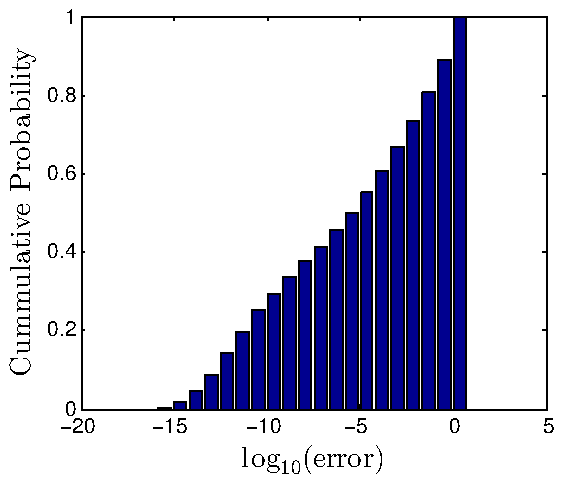
\includegraphics[width=0.3\linewidth]{CProb50.pdf}
        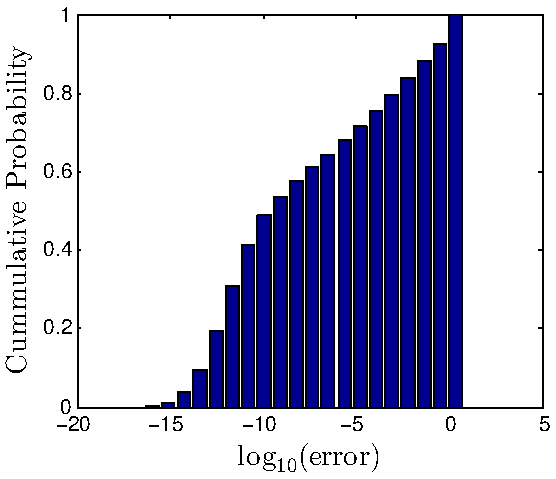
\includegraphics[width=0.3\linewidth]{CProb100.pdf}
        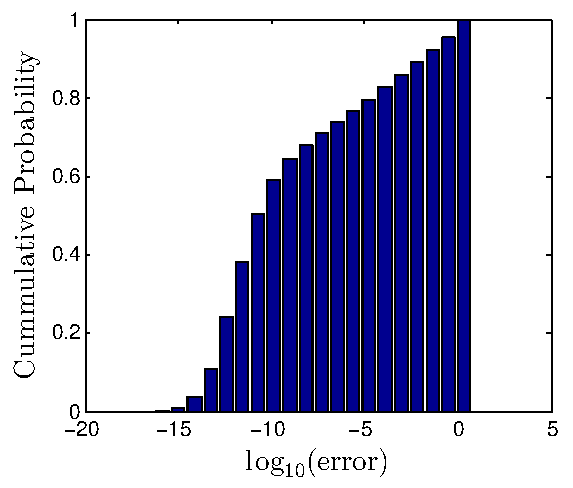
\includegraphics[width=0.3\linewidth]{CProb200.pdf}
    \end{centering}
    \caption{\label{fig:PEerrorhist}
     Cumulative distribution function of probability that PE error is less than $x$ after $150$ updates for $m=50$ (left) $m=100$ (middle) $m=200$ (right).
    }
\end{figure*}

\section{Additional Numerics}
\begin{figure}
    \begin{centering}
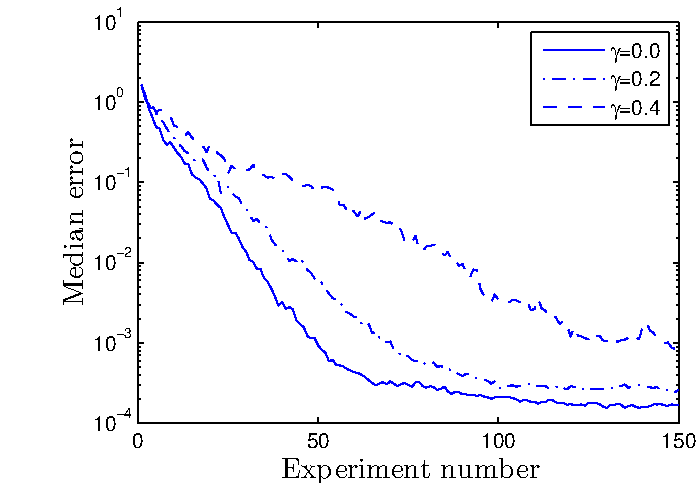
\includegraphics[width=0.6\linewidth]{Gammascale.pdf}
    \end{centering}
    \caption{\label{fig:gamma}
Errors in inference for phase estimation with different levels of un-modeled noise, $\gamma$, for $T_2=1000$.  In each instance the initial state was taken to be a fixed, but unknown, eigenstate of the Hamiltonian.  The median was found for $100$ randomly chosen values of the eigenphase of this fixed initial eigenstate.
    }
\end{figure}

Our algorithm is similarly robust against~\emph{uncharacterized noise sources} as well.  We demonstrate this in~\fig{gamma} wherein we introduce depolarizing noise of strength $\gamma$ to our experimental system, but do not include such noise in the likelihood function.  For example, with $\gamma=0.4$, the measurement outcome of phase estimation is replaced with a random bit with probability $40\%$.  We find that while the inclusion of such noise causes the error decay exponent to shrink as roughly $0.17e^{-3.1\gamma}$ it does not prevent our algorithm from learning at an exponential rate (until depolarizing noise becomes significant).  This illustrates that our method for phase estimation can continue to work even in the presence of noise sources that are both strong and uncharacterized.





\end{document}